\documentclass{../../text-style}

\texttitle{Лекция 7: Управление проектами, часть 2: планирование и управление}

\begin{document}

\maketitle
\thispagestyle{empty}

\attribution{Тимофей Александрович Брыксин, бывш. доцент кафедры системного программирования СПбГУ}

Одним из основных факторов успешного выполнения проекта является составление хорошего графика работ, который обладает следующими характеристиками:

\begin{itemize}
    \item \emph{основывается на детальной декомпозиции.} Он учитывает все виды деятельности, которые вы запланировали, на которые вы разбили ваш проект;
    \item \emph{содержит все задачи в правильном порядке.} Почти всегда задачи в проекте взаимосвязаны друг с другом, поэтому их необходимо выстроить в правильной последовательности;
    \item \emph{учитывает сторонние ограничения, не зависящие от команды}, т.е. учитывает разного рода события, которые происходят извне;
    \item \emph{может быть завершен вовремя при наличии нужных ресурсов.} Если у вас есть график, в котором все подробно и детально расписано, но у него точка завершения по времени через месяц после дедлайна, то это не очень хороший график;
    \item \emph{направлен на достижение целей проекта.}
\end{itemize}

Построение такого плана включает в себя ряд шагов, которые мы и разберём в этой лекции.

\section{Планирование проекта}

Планирование проекта предполагает множество взаимосвязанных итераций, итогом которых выступает единый сводный план. Рассмотрим основные задачи планирования (первые три из них мы разбирали в прошлый раз).

\begin{enumerate}
    \item \emph{Определение сути проекта.} В первую очередь необходимо понять, \enquote{что вы будете производить}, прежде чем решать, \enquote{как это производить}. Вы уточняете и детализируете цели и результаты проекта.
    \item \emph{Разработка стратегии управления рисками.} На этом этапе вы выявляете препятствия, которые могут возникнуть в ходе реализации проекта, оцениваете их, а затем определяете варианты действий по их устранению.
    \item \emph{Декомпозиция проекта.} Невозможно анализировать сложную систему, рассматривая ее как единое целое. Поэтому, как правило, требуется сначала разбить ее на части (подсистемы) и лишь потом проводить анализ.
    \item \emph{Выявление зависимостей между задачами.} При планировании задач необходимо учитывать взаимосвязи между ними. Например, вы не можете начать писать документацию, пока не будут разработаны компоненты системы. В свою очередь проект не будет принят заказчиком, пока не будет написана документация. Поэтому необходимо определить, какие связи есть между задачами, в каком порядке их нужно выстроить.
    \item \emph{Оценка задач.} Для каждой задачи определяются объем работы и ее длительность, которая измеряется в человеко-часах/-днях/-неделях.
    \item \emph{Создание и оценка плана работ.} После того, как вы разбили ваш проект на задачи, установили последовательность их выполнения и оценили каждую из них, вы составляете план. Здесь уже вычисляются сроки выполнения всего проекта, указываются запланированные даты начала и завершения. Но следует учитывать, что первоначальный план, скорее всего, не будет соответствовать имеющимся ограничениям по производственным ресурсам, времени или каким-нибудь другим параметрам. Поэтому есть еще пункт 7.
    \item \emph{Распределение и оптимизация ресурсов.} Планирование~--- это итеративный процесс. С первого раза его очень сложно сделать правильно, поэтому эта стадия предполагает серьезную корректировку всего графика, который был построен до этого. Задачи перепланируются с целью оптимизации распределения людей и ресурсов, используемых в проекте. Вы получаете новую информацию, основываясь на которой можете более точно спланировать вашу деятельность.
\end{enumerate}

Таким образом, эти шаги генерируют довольно много информации, необходимой для понимания того, как будет выполняться проект. Эта работа сильно итеративная, с первого раза вряд ли сразу получится получить хороший план.

\subsection{Матрица зависимостей}

\begin{center}
    \begin{tabularx}{\textwidth} { 
        | >{\centering\arraybackslash}X 
        | >{\centering\arraybackslash}X 
        | >{\centering\arraybackslash}X | }
        \hline
        Операция                                  & Непосредственно предшествующие операции & Длительность \\
        \hline
        A. Установка компьютеров                  &~---                                     & 1            \\
        \hline
        B. Протяжка сети                          &~---                                     & 2            \\
        \hline
        C. Настройка сети                         & A, B                                    & 3            \\
        \hline
        D. Установка программного обеспечения     & C                                       & 1            \\
        \hline
        E. Разработка регламента использования ПО &~---                                     & 4            \\
        \hline
        F. Обучение пользователей                 & D, E                                    & 3            \\
        \hline
    \end{tabularx}
\end{center}

После того как вы определили задачи проекта, необходимо определить связи между ними. Зависимости между задачами влияют на даты планируемого начала или завершения задач. Наиболее распространенный тип связи~--- это когда работа B не может начаться раньше, чем закончится работа А. Например, задача \enquote{интегрировать модуль Х} не может начаться, пока не завершится задача \enquote{реализовать модуль Х}.

Матрица зависимостей представляет собой простой, но эффективный метод обнаружения связей между задачами. Вы выписываете все задачи, нумеруете их каким-нибудь уникальным идентификатором и пишите, за какой задачей должна выполняться конкретная задача.

Но следует учитывать, что когда у вас есть большое количество задач и между ними сложные зависимости, то такая форма представления может оказаться ненаглядной. Чаще всего используют так называемый сетевой график.

\subsection{Сетевой график}

Сетевой график~--- это модель, отражающая зависимость и последовательность выполнения задач. Этот график передает ту же самую информацию, что и матрица зависимостей, но он более наглядный: на нём гораздо более явны потенциальные проблемы и возможности для их решения. Например, вначале часто удобно бывает построить таблицу, а потом по ней уже график.

Основными параметрами сетевого графика являются работа и событие. Под работой подразумевается любой процесс, требующий затраты времени. Событие~--- это промежуточный или окончательный результат одной или нескольких работ, необходимый для начала других работ. Событие совершается после выполнения всех работ, входящих в него. Работу на сетевом графике изображают одной сплошной стрелкой. Продолжительность работы в единицах времени (часы/дни/недели) и наименование работ обычно пишут рядом со стрелкой. Каждое событие изображается кружком и нумеруется.

\begin{center}
    \begin{tikzpicture}
        [every path/.style={font=\ssmall}]

        \node[shape=circle,draw=black] (1) at (0,0) {1};
        \node[shape=circle,draw=black] (2) at (2.5,1.5) {2};
        \node[shape=circle,draw=black] (3) at (2.5,-1.5) {3};
        \node[shape=circle,draw=black] (4) at (5,0) {4};
        \node[shape=circle,draw=black] (5) at (8,0) {5};
        \node[shape=circle,draw=black] (6) at (11,0) {6} ;
        
        \path [->](1) edge node[align=center] {A. Установка компьютеров\\ \textit{1 день}} (2);
        \path [->](1) edge node[align=center] {B. Протяжка сети\\ \textit{2 дня}} (3);
        \path [->,dashed](3) edge node[] {} (2);
        \path [->](2) edge node[align=center] {C. Настройка сети\\ \textit{1 день}} (4);
        \path [->](4) edge node[align=center,below=5pt] {D. Установка программного\\ обеспечения\\ \textit{1 день}} (5);
        \path [->](5) edge node[align=center,below=5pt] {F. Обучение\\ пользователей\\ \textit{1 день}} (6);
        \path [->](1) edge[bend right=70] node[align=center,below] {E. Разработка регламента\\использования ПО\\ \textit{1 день}} (5);
    \end{tikzpicture}
\end{center}

Здесь есть два важных момента.

\begin{enumerate}
    \item Задачи, которые попадают в этот график~--- это те самые задачи, которые вы получили при декомпозиции, которые вы потом будете \enquote{делать руками}. Т.е. тут не пишутся задачи, которые находятся в промежуточных узлах и обобщают задачи уровня ниже. Сюда заносятся только те задачи, которые вы реально будете делать, которые вы будете оценивать, из которых будет строиться все состояние.
    \item Сетевой график должен отражать только зависимости между задачами. Не надо строить этот график, учитывая те ресурсы, которые у вас есть. Просто забудьте о них. Представьте, что у вас есть неограниченное число людей, денег и т.д. Изменение сетевых графиков из-за ограничений ресурсов является наиболее распространенной ошибкой при построении такого рода диаграмм. Тот факт, что не хватает людей или других ресурсов для одновременного выполнения нескольких задач, не имеет значения. Независимо от ресурсов, задачи все равно должны выполняться в том же порядке.
\end{enumerate}

\subsubsection{Основные правила разработки сетевого графика}

При разработке сетевого графика целесообразно придерживаться следующих правил:

\begin{itemize}
    \item Ни одна операция не может быть начата, пока все предшествующие связанные с ней операции не будут выполнены.
    \item Стрелки в сетевом графике отображают отношения предшествования и следования. На рисунке стрелки могут пересекаться.
    \item Каждая операция должна иметь свой собственный номер.
    \item Номер последующей операции должен быть больше номера любой предшествующей операции.
    \item Образование петель недопустимо (другими словами, не должно происходить зацикливания хода выполнения установленного набора операций).
    \item Условные переходы от одной операции к другой не допускаются (имеется в виду определение последовательности хода выполнения операций условиями типа: \enquote{Если будет достигнут успех, сделайте то-то...; если нет~--- ничего не предпринимайте}).
\end{itemize}

При включении любой операции в сетевой график необходимо определить для нее три отношения. Эти отношения могут быть определены в результате ответов на следующие три вопроса:

\begin{itemize}
    \item Какие операции должны быть завершены непосредственно перед этой операцией?
    \item Какие операции должны следовать непосредственно за этой операцией?
    \item Какие операции могут выполняться во время выполнения этой операции? Какие операции можно назвать параллельными данной?
\end{itemize}

\subsubsection{Внешние события и майлстоуны}

Часто на сетевом графике бывает удобно указывать также внешние для проекта события и ключевые точки (майлстоуны) проекта. Они не требуют никакого времени и не влияют на продолжительность путей в сетевом графике, однако часто удобны для синхронизации хода работ. К ним можно отнести точки начала и завершения работ, даты выпуска версий ПО, события получения денег от заказчика или что-то ещё.

\subsection{Оценка задач}

После того, как вы нарисовали такой график, выяснили, что от чего зависит, нужно каждую задачу аккуратно оценить. Оценивают их обычно по времени. Только необходимо понимать, что это не фактическое время выполнение задачи, а время от начала реализации этой задачи до получения конечного результата. Т.е. если вы сделали задачу за 20 мин, а потом запустили тесты, чтобы проверить, и они, например, идут два дня, то время выполнения данной задачи будет не 20 мин, как это ошибочно можно полагать, а 2 дня и 20 мин. Это очень важный момент, поэтому вы должны четко представлять, что является конечным результатом конкретной задачи.

Есть еще такое понятие, как объем работы, и это именно то, в чём скорее всего будут оценивать задачи технические специалисты. Для того, чтобы конвертировать объём работы в календарное время, вам нужно знать продуктивность людей, которые будут делать эту задачу. Есть очень простая формула:

$$\textup{Длительность работ} = \frac{\textup{Объём работ}}{\textup{Производительность}}$$

Но эту формулу очень сложно применять, поскольку, как правило, вы не знаете ни числитель, ни знаменатель. Вы, конечно, можете примерно прикинуть и то, и другое, но с погрешностью, и эта погрешность может оказаться довольно большой.

Все понимают, что разные программисты пишут код по-разному, с различной скоростью. И здесь нельзя просто взять и посчитать среднюю производительность. Представьте, что у вас есть четыре программиста, у первых двух высокая продуктивность, у вторых двух низкая. Вы посчитали среднюю производительность, и затем задача досталась одному из них. Если она попала первым двум программистам, то они сделают ее быстрее, а если она попала другим двум, они просто не успеют. Ну и не стоит забывать, что один и тот же человек работает с различной производительностью в разные дни. Это сильно усложняет точную оценку, но в некотором приближении пользоваться этим всё равно приходится. Тут многое зависит от того, насколько хорошо вы знаете свою команду, а команда знает проект, который вы планируете.

Ещё при конвертации объёма работ во время не стоит рассчитывать, что каждый разработчик будет стабильно выдавать вам по 8 часов продуктивной работы каждый день. Продуктивно писать код по 8 часов в день довольно сложно, разработчики так или иначе оказываются вовлечены в разные совещания, планирование и оценку, проектирование, да и просто могут помогать коллегам с их задачами. Правильные коэффициенты тут тоже выясняются обычно опытным путём и сильно зависят от конкретных людей и принятых процессов.

Отдельная сложность при планировании работы людей, занятых на нескольких проектах сразу. Сложность совмещения проектов заключается в переключении контекстов. Разработка ПО~--- крайне творческая задача, часто требующая серьёзного погружения в предметную область, имеющийся код и особенности задачи. Если человека постоянно дёргать туда-сюда между проектами и задачами, он просто большую часть времени будет тратить на переключение между ними, а на собственно решение задач будет оставаться гораздо меньше восьми часов в день. Ну и в чём-то схожая ситуация с людьми, занятыми не на полную ставку (разного рода стажёры и т.п.), им может приходиться тратить какое-то время на синхронизацию с тем, что было сделано другими членами команды в их отсутствие.

Вот некоторая статистика, которую авторы статьи Astromskis et al. Patterns of Developers Behaviour: A 1,000-hour Industrial Study, 2017 собрали по шестерым разработчикам одной компании, занимавшейся разработкой встроенного ПО на C++, наблюдая за их действиями более тысячи рабочих часов:

\begin{center}
    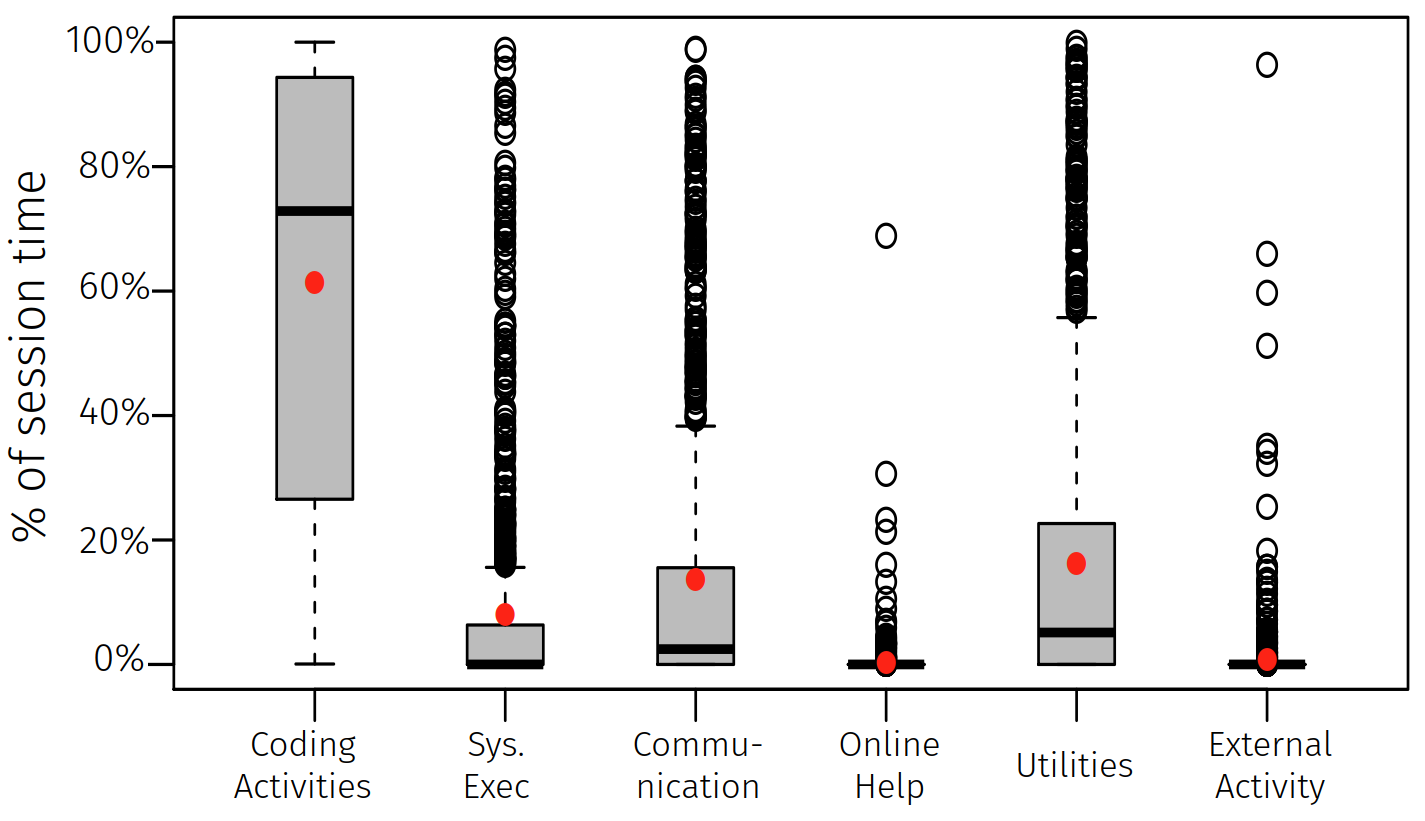
\includegraphics[width=0.95\textwidth]{timeSpentDuringWorkingSession.png}
    \attribution{Astromskis et al. Patterns of Developers Behaviour: A 1,000-hour Industrial Study, 2017}
\end{center}

Авторы разбили всю деятельность на работу с кодом (чтение или написание, не важно), запуск разрабатываемой системы, коммуникацию с коллегами (посредством мессенджеров, живое общение не входило), поиск информации в интернете, использование разного вспомогательного ПО, и деятельность, не относящуюся к работе. Статистика собиралась только во время рабочих сессий, то есть когда разработчик сидел за компьютером и что-то активно делал.

Выяснилось, что на собственно работу с кодом уходило порядка 60\% рабочего времени, 8\% на запуск системы (скорее всего, для тестирования), 16\% на вспомогательные инструменты (данные подготовить или что-то такое), 2\% (всего!) на поиск справки в интернете, 14\% на коммуникацию, 1\% на нерабочие активности (новости почитать, например). Статистику нельзя обобщать на все команды и все компании, но становится понятно, что даже то, что мы считаем плотной работой, на самом деле довольно сильно разбавлено вспомогательными процессами.

А если посмотреть на статистику по рабочему времени всего, а не только активной работы, станет ещё понятнее, почему человеко-день в 8 часов~--- это заведомый провал:

\begin{center}
    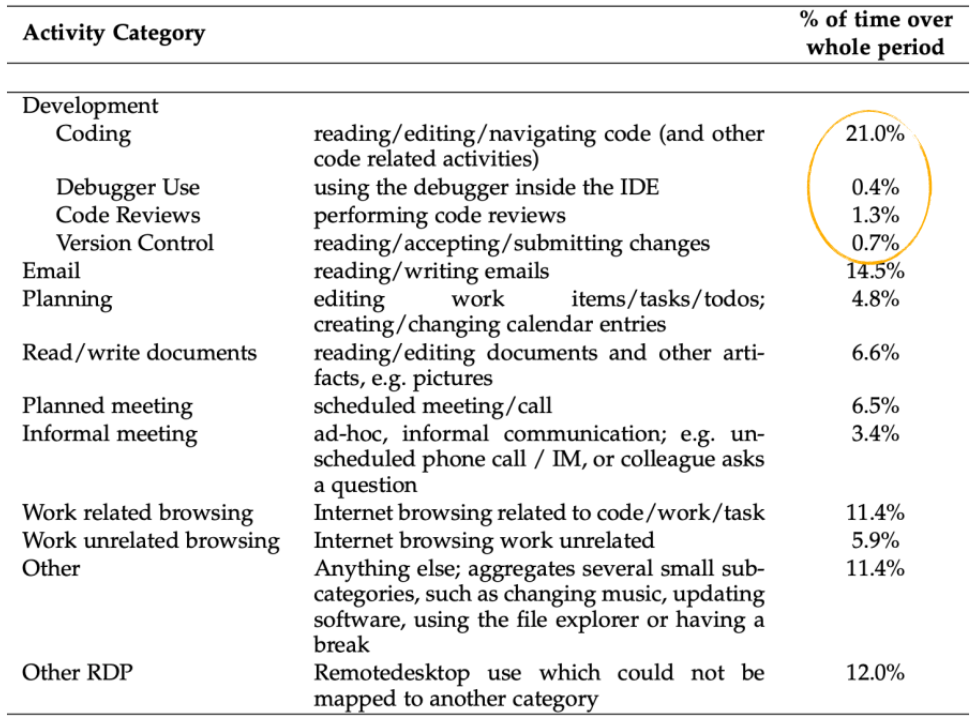
\includegraphics[width=0.7\textwidth]{timeSpentTotal.png}
    \attribution{Meyer et al. The work life of developers: Activities, switches and perceived productivity, 2017}
\end{center}

Причём это нормальная, честная и хорошая работа.

\subsection{Оценка графика работ}

Предположим, что вы как-то оценили все ваши задачи. Теперь вы хотите построить общий график и вычислить сроки выполнения всего проекта. Делается это на основе того же самого сетевого графика, только теперь он немного видоизменяется.

\begin{center}
    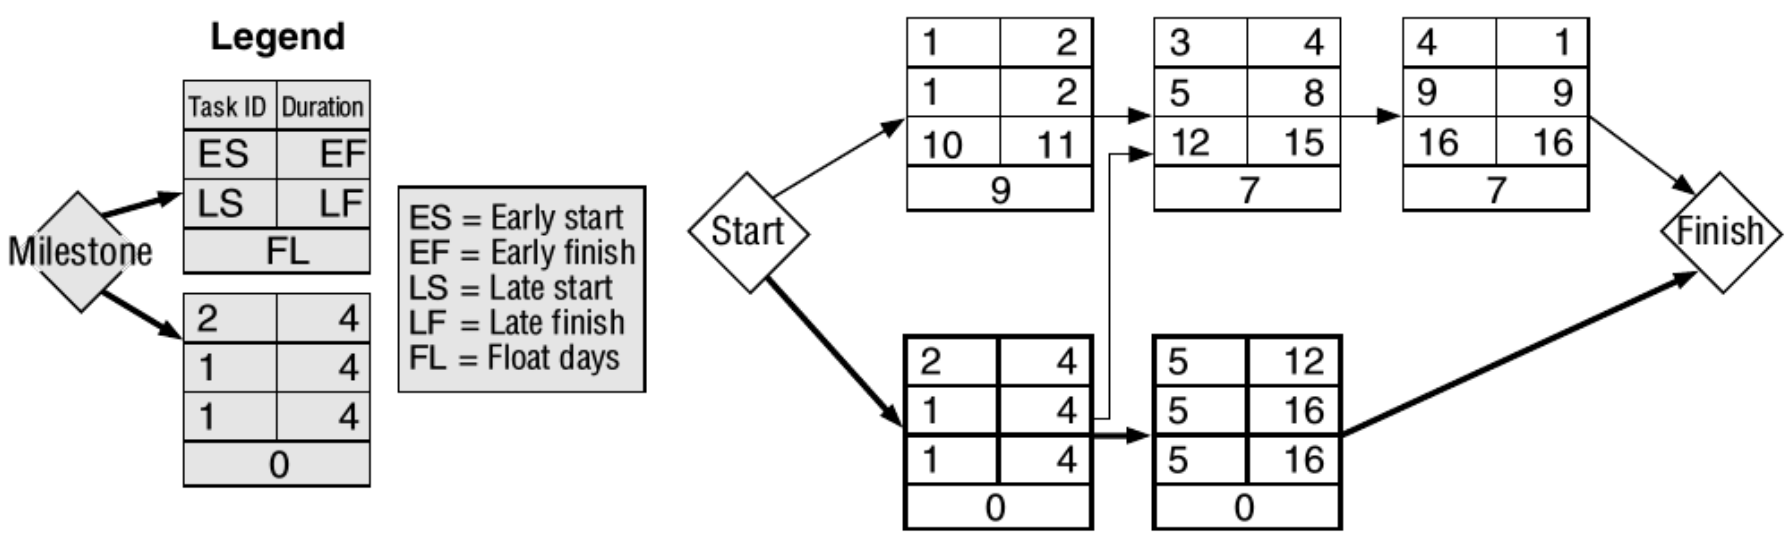
\includegraphics[width=0.95\textwidth]{graphEstimate.png}
\end{center}

По сути, справа нарисован сетевой график. Табличка слева~--- это легенда, которая просто показывает, что эти кубики значат. Здесь используются следующие понятия.

\begin{itemize}
    \item \emph{Раннее начало (ER)}~--- это самая ранняя дата, с которой может начаться задача. Т.е. эта величина показывает время, раньше которого задача не может быть начата.
    \item \emph{Раннее окончание (EF)} определяется суммой раннего начала и продолжительности рассматриваемой задачи.
    \item \emph{Позднее начало (LS)}~--- это самая поздняя дата, когда задача может быть начата без задержки завершения проекта. Т.е. эта величина показывает время, позже которого задача не может быть начата без увеличения продолжительности всего проекта.
    \item \emph{Позднее окончание (LF)} вычисляется как сумма позднего начала и продолжительности рассматриваемой задачи.
\end{itemize}

Первая строчка элемента сетевого графика: слева идентификатор (номер задачи), а справа~--- длительность. Т.е. глядя на первый прямоугольник, вы понимаете: задача 1 длительностью в 2 единицы. Во второй/третьей строчке записываются раннее/позднее начало и раннее/позднее окончание.

Теперь о том, как это все вычислить. В самом начале у вас все ячейки пустые, кроме первой строки. Идентификатор задач и их длительность вы знаете.

\subsubsection{Шаг 1. Прямой проход}

Он называется так потому, что вычисления начинаются с исходного события и продолжаются до тех пор, пока не будет достигнуто завершающее событие. Прямой проход помогает вам определить раннее начало и раннее окончание для каждой задачи. Пойдем по порядку:

\begin{enumerate}
    \item Первая задача. Она занимает два дня. Значит, это первый и второй день. Следовательно, early start = 1, early finish = 2. Идем дальше в задачу 2.
    \item Вторая задача. Она ни от чего не зависит. Значит, ее можно начать выполнять сразу же (в первый день). Длительность = 4, поэтому early finish = 4.
    \item Третья задача. Она не может начаться раньше, чем завершится задача 2. Поэтому у нее early start = 5, early finish = 8.
\end{enumerate}

И так далее вы заполняете эти оптимистичные оценки.

\subsubsection{Шаг 2. Обратный проход}

Обратный проход  определяет позднее начало и позднее окончание. Цель обратного прохода~--- пройтись в обратном направлении от даты окончания проекта, чтобы определить, насколько поздно любая задача может начаться и завершиться. Т.е. вы берете последнюю дату и смотрите: \enquote{если мы в этот момент все закончим, то когда должна начать выполняться последняя задача?}. И отнимаете от нее, сколько она длится. Затем смотрите, от кого она зависит. И таким образом идёте в самое начало. 

\subsubsection{Шаг 3. Вычисление резервов}

Резерв (float) вычисляется как разница между поздним и ранним началом. Он показывает, какой у вас есть запас времени между этими двумя величинами. Значение резерва вполне может быть отрицательным значением: это значит, что вы уже не успеваете к обозначенной дате завершения проекта.

\subsection{Критический путь}

Одной из ключевых особенностей построенного графика является критический путь. Это такой путь, у которого все задачи в ячейке резерва  имеют ноль или отрицательные значения. Другими словами, критический путь~--- путь от исходного до завершающего события, имеющий наибольшую длину (продолжительность) из всех путей. Критический путь является одним из показателей жизнеспособности графика. Это объясняется тем, что он демонстрирует минимальное время, которое займет проект. Поэтому увеличение длительности задач, лежащих на критическом пути, увеличивает общую продолжительность проекта. Соответственно, сокращение этих работ приводит к общему сокращению срока выполнения проекта. Заметим, что в сетевом графике может быть несколько критических путей. На графике выше критический путь выделен утолщенными линиями.

\subsection{Другой формат представления сетевого графика}

\begin{center}
    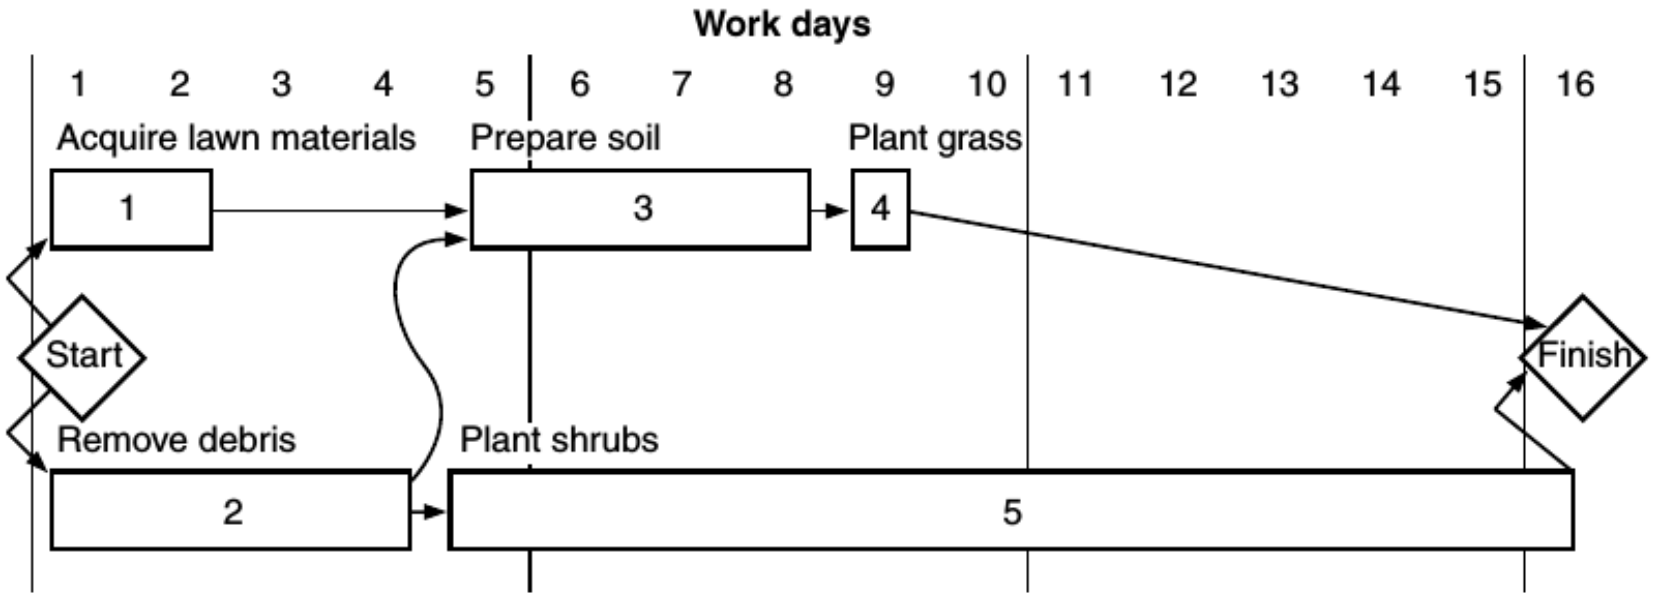
\includegraphics[width=0.95\textwidth]{otherGraphFormat.png}
\end{center}

Такой график еще более наглядный, но его сложно строить \enquote{вручную} и он занимает много места. Поэтому если у вас много задач, для построения таких графиков пользуйтесь специализированными инструментами.

\subsection{Диаграмма Гантта}

Диаграмма Гантта~--- это популярный тип столбчатых диаграмм, который используется для иллюстрации плана, графика работ по какому-либо проекту. Она представляет собой отрезки, размещенные на горизонтальной шкале времени. Задачи, составляющие план, размещаются по вертикали. Каждый отрезок соответствует отдельной задаче. Начало, конец и длина отрезка на шкале времени соответствуют началу, завершению и длительности задачи.

\begin{center}
    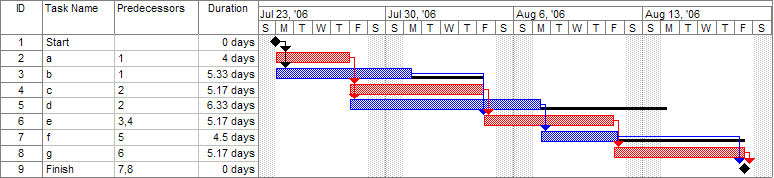
\includegraphics[width=0.95\textwidth]{ganttChart.png}
\end{center}

Важно то, что здесь тоже все делается без учета ресурсов, т.е. вы показываете только зависимости между задачами. Эта диаграмма очень часто используется, поскольку она крайне наглядная и ее можно рисовать где угодно. Например, часто для этого используют Excel/Google Spreadsheets. 

\begin{center}
    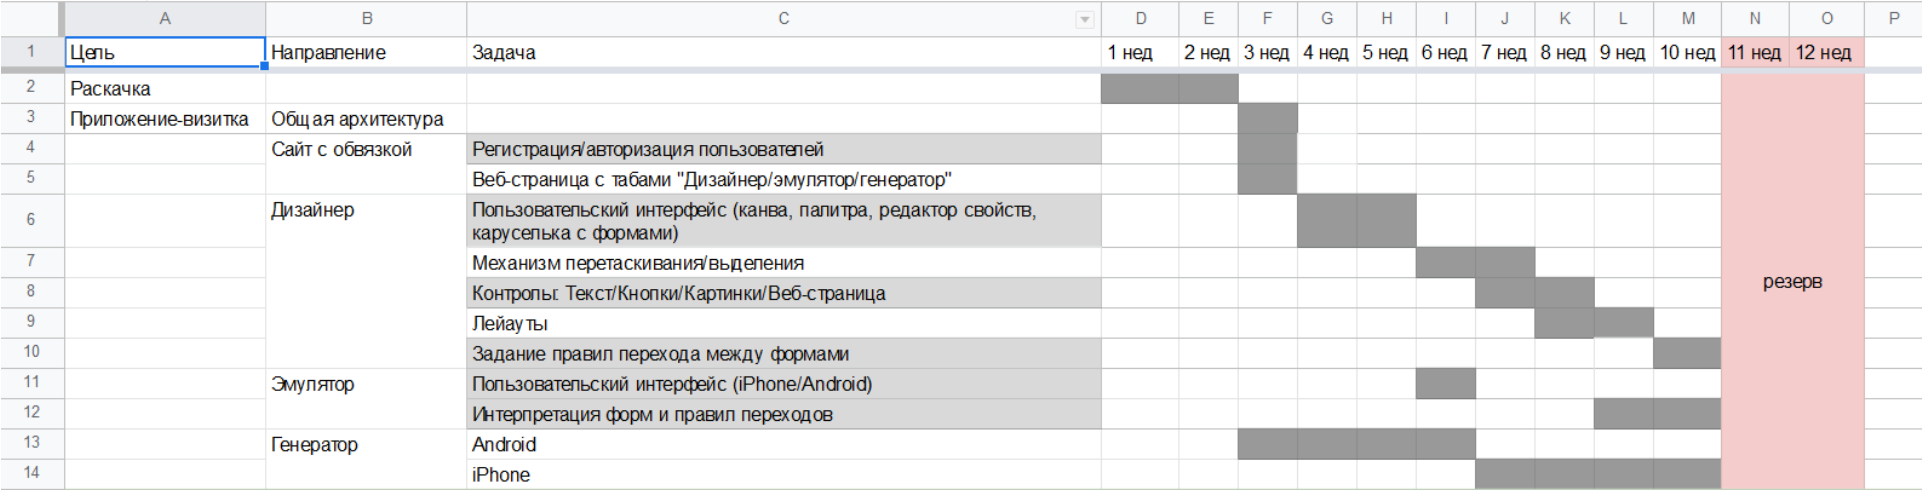
\includegraphics[width=0.95\textwidth]{ganttChartExample.png}
\end{center}

Единственная проблема, которая здесь будет~--- это перемещение задач. Т.е. если вы поняли, что вы сначала сделали задачу 4, а потом задачу 3, то просто поменять строки местами не получится. Вам еще потом придется сдвигать закрашенные ячейки.

\subsection{Диаграмма Гантта с указанием ресурсов}

\begin{center}
    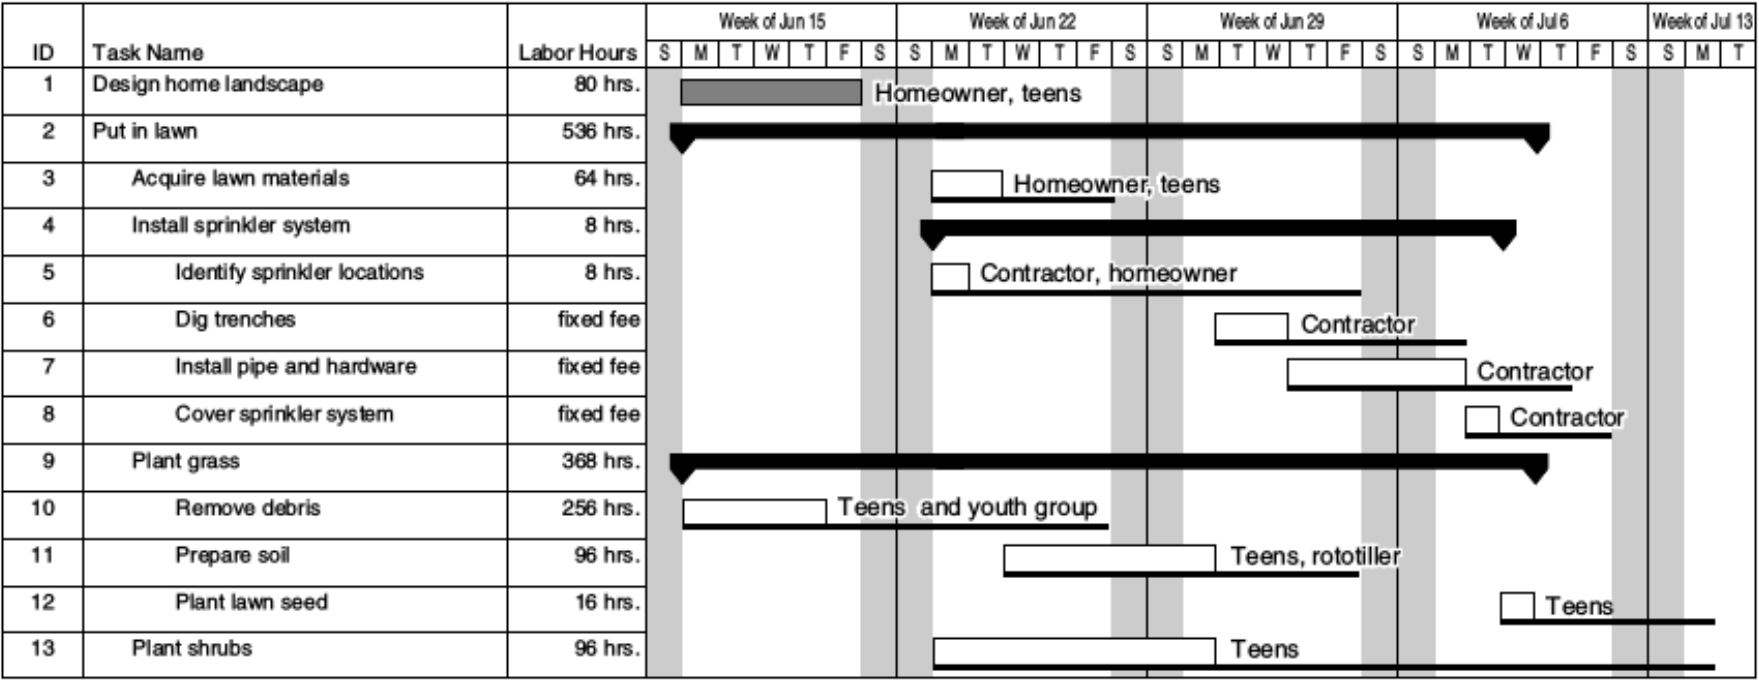
\includegraphics[width=0.95\textwidth]{ganttChartWithResources.png}
\end{center}

\begin{center}
    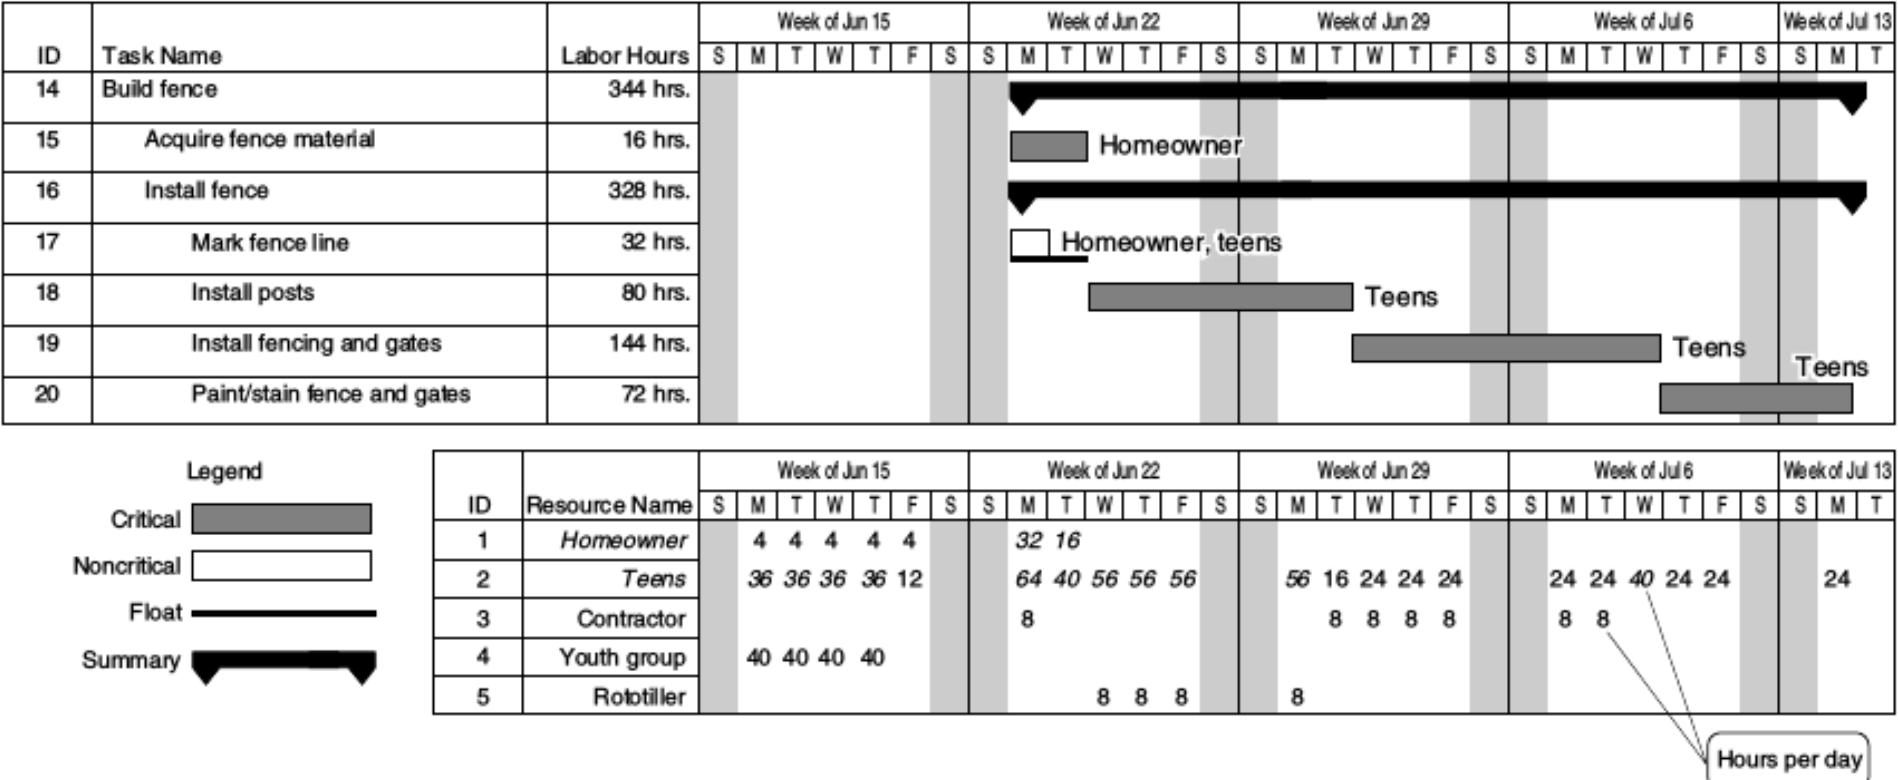
\includegraphics[width=0.95\textwidth]{ganttChartResourceUtilization.png}
\end{center}

На этой диаграмме еще указывается дополнительная информация. Здесь указаны составные задачи проекта (такие как \enquote{Put in lawn}), т.е. задачи, которые разбиваются на несколько других (промежуточный узел дерева декомпозиции). Жирной чёрной линией указан резерв (например, у задачи \enquote{Remove debris}), но в целом указывать его не обязательно.

Также на обычной диаграмме Гантта вообще нет информации о людях. Т.е. не указывается, кто делает какую задачу. А здесь эти сведения добавляют. Такую диаграмму можно достаточно быстро читать и в ней закладывается довольно много информации.

\subsection{Оптимизация ресурсов}

Итак, вы построили начальный план. Он потому и начальный, что он в принципе не подразумевает никакого распределения ресурсов. Начальный план показывает то, как задача была бы сделана в идеальном случае, но такого почти никогда не бывает. Поэтому этот план нужно оптимизировать в соответствии с ресурсами, которыми вы располагаете. Ресурсы~--- это люди, оборудование, материалы и т.п.

Здесь есть два понятия: перегруженность (overallocation) и недозагруженность (underallocation). Перегруженность означает, что вы пытаетесь перегрузить ваши ресурсы работой. Например, у вас есть один программист и вы ему нарисовали диаграмму, где он должен параллельно заниматься пятью задачами. Разумеется, он за один день не сделает 5 задач, длительность каждой из которых составляет один день. Он будет делать их 5 дней, и ваш график поедет. Перегруженность плоха ещё и потому, что когда вы перегружаете человека, он быстро устаёт и переутомляется, у него падает производительность.

Другая сторона проблемы~--- это недозагруженность: ситуация, при которой есть люди, которые ничем не заняты. Понятно, что это тоже плохо, поскольку вы просто теряете деньги, плюс это почти всегда сказывается негативно на большинстве людей. Чаще всего программисты работают не за зарплату. Программисты хотят решать интересные задачи, и в отсутствии достойной работы им реально становится скучно. Хорошие программисты долго на таких местах обычно не задерживаются. А в некоторых странах вот даже такое бывает: \url{https://www.personneltoday.com/hr/interparfums-boreout-case/} (дата обращения: 27.03.2023г).

Смотря на самую последнюю версию диаграммы Гантта, вы можете построить следующий график:

\begin{center}
    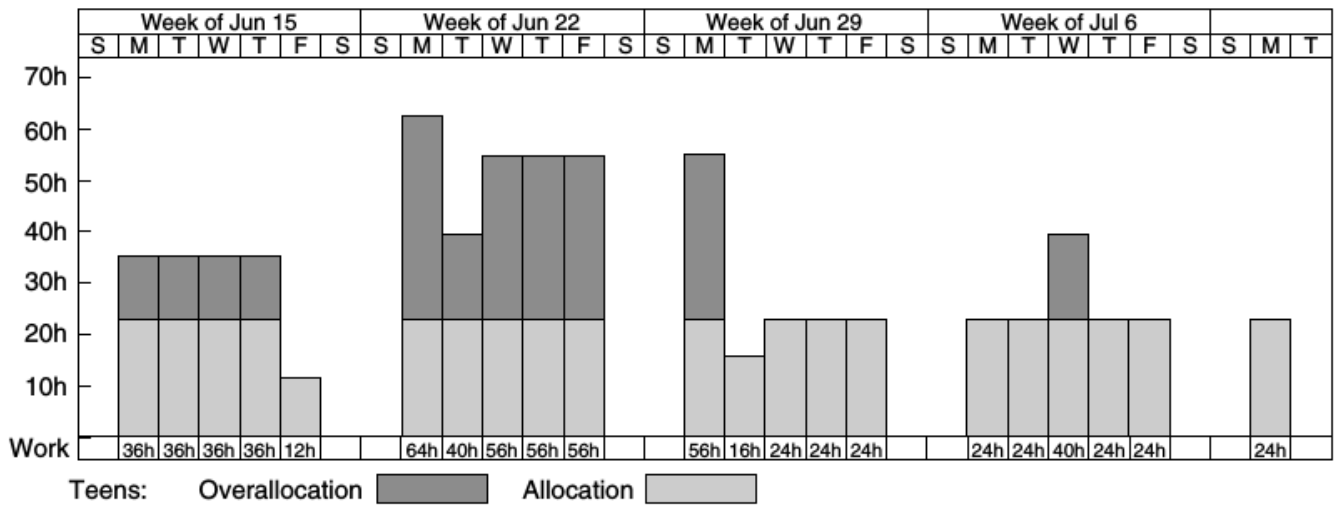
\includegraphics[width=0.7\textwidth]{resourceAllocation.png}
\end{center}

Видно, что в первый день вам нужно 36 человеко-часов, во второй 36 ч/ч, а в пятый 12 ч/ч. Человек в день должен работать по 8 часов, не более. В предыдущей таблице было три разработчика. Поэтому здесь allocation отмечено как 24 ч/ч~--- сколько они в сумме могут отработать за один день. Это пример несбалансированного графика работ.

Глядя на такие диаграммы, вы понимаете, что у вас есть пики (когда вы пытаетесь сделать слишком много), их имеет смысл выравнивать. Чтобы этого добиться, вы просто пытаетесь двигать ваши задачи в соответствии с тем резервом, который у них есть. Если у некоторой задачи резерв равен 9, то вы ее можете двигать в пределах девяти единиц времени. Вы можете отложить ее на 9, но она все равно не повлияет на конечный дедлайн. Т.е. резерв вам позволяет перемещать эти задачи по времени. В нашем примере, надо сдвигать задачи с первых четырёх дней на пятый. В этом примере это всё равно не позволит загрузить всех равномерно и сделать всё вовремя, но как первый шаг это вполне стоит того. Далее, если время является ключевым фактором, нужно искать возможность добавить людей на критические задачи или как-то иначе выровнять график. Но это тоже не всегда просто сделать: программисты~--- не укладчики кирпичей, которых можно без проблем заменять одного на другого. В итоге получается жонглирование большим количеством параметров, к которому нужно подходить очень аккуратно.

\subsection{Типичные ошибки при оценке проектов}

\textbf{Оценку делали не те люди. Мало опыта, непонимание техник оценивания.} Оценки должны делать нужные люди. Важно, чтобы это были те люди, которые хорошо знают предметную область. Независимо от того, какие методы используются, оценка всегда основывается на понимании работы, которую предстоит выполнить. Также к оценке стоит привлекать людей, которые будут фактически выполнять эту работу. Они имеют лучшее понимание своих способностей, к тому же, если человек знает, что ему предстоит делать данную задачу, то он ответственнее подойдет к ее оценке. Но при этом, если у вас нет никакого опыта оценивания, то первую оценку, скорее всего, вы сделаете очень плохо. Со временем, если вы будете анализировать и использовать свой опыт, вы научитесь это делать более точно.

\textbf{Слишком быстрый ответ и оценка в условиях недостаточной информации.} Никогда не давайте быстрых ответов. Вы всегда что-нибудь забудете, всегда оцените более оптимистично, чем хотелось бы. Поэтому есть несколько стратегий, как с этим бороться.

\begin{itemize}
    \item Каким-то образом откажитесь от ответа, но это не всегда оказывается возможным.
    \item Начните задавать вопросы, уточнять некоторые моменты. Когда вы получите больше информации, вы сможете точнее сделать оценку. Но, скорее всего, информации у того человека, который вас это спрашивает, нет. Поэтому после несколько вопросов, на которые вам не смогли дать ответ, менеджер сам поймет, что слишком много неизвестных, чтобы дать сейчас точную оценку.
    \item Попробуйте оценить задачу максимально точно, а потом умножьте ее на два. А затем еще раз на два. Это тот коэффициент, который, скорее всего, будет похож на правду. Т.е. если вы про что-нибудь не знаете или забудете, то благодаря этому коэффициенту вы с большой долей вероятности все туда уложите.
\end{itemize}

\begin{center}
    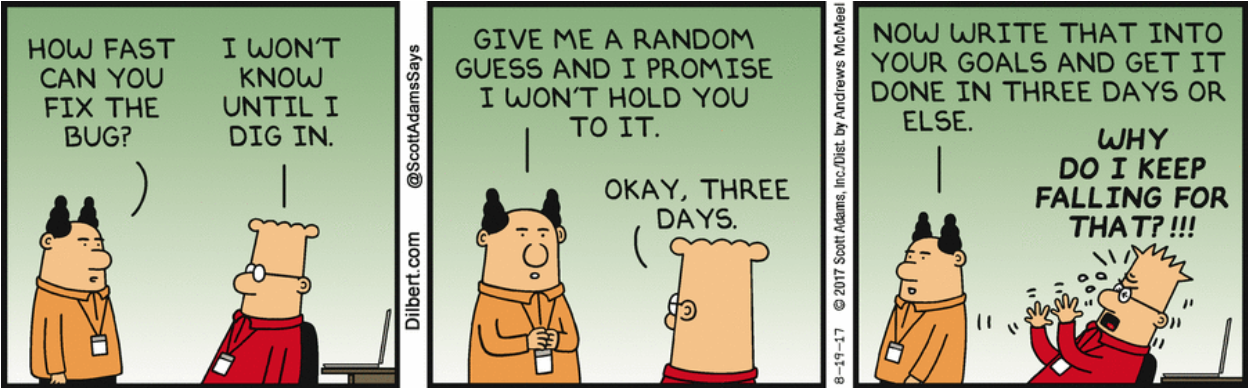
\includegraphics[width=0.7\textwidth]{dilbertEstimation.png}
\end{center}

\textbf{Забыли про риски и прочие буферы.} На одной из прошлых лекций мы говорили о том, что противодействие рискам стоит денег. Скорее всего, если вы умножите вашу изначальную оценку на 4, то этот бюджет на риски и прочие буферы туда просто войдут автоматически, хотя бы частично. Но если вы этого не делаете, то проведите переоценку рисков, продумайте, как реализация и интеграция этой задачи повлияет на другие задачи и проект в целом.

\textbf{Забыли про налоги.} У вас есть диаграммы, вы посчитали количество человеко-часов, умножили их на зарплату. Допустим, что вы учли подоходный налог, но при этом забыли про все остальные налоги, половину бюджета вы просто выкинули. С человека государство берет 13\%, но с компании гораздо больше, до 54\%. Если это не заложить в бюджет, вам придется это платить из собственного кармана.

\textbf{Забыли про расходы на \enquote{административный аппарат}.} Еще один пункт, который включается в общую сумму проекта. Вы считаете затраты по задачам, которые делают программисты. Вы учитываете их зарплаты, подсчитываете общий бюджет, свою зарплату вы тоже скорее всего посчитали. Но есть еще уборщица, водитель, отдел кадров, менеджеры над вами, бухгалтеры, ген. директор, его секретарь и т.д. Назовем их \enquote{административным аппаратом}, и им тоже нужно платить деньги. Поэтому вы должны добавить к общей сумме проекта еще некий процент на эти издержки. Если у вас компания маленькая (10–20 чел), то процент будет небольшой (5–10\%). Если у вас большая компания (300–400 чел), то накрутка может доходить до 30–40\%. И заказчики платят эти деньги, потому что крупная компания считается более надёжной, не совершает \enquote{детских ошибок} и т.п.

\textbf{Забыли про отпуск.} Вы берете ваш график и рассчитываете для каждого человека: 8ч в день => 40ч в неделю => x часов в год. Но потом оказывается, что работа у вас вовремя не заканчивается, поскольку 1/12 вы куда-то потеряли. Отпуск~--- это то время, когда человек освобождается от работы для отдыха. Это нужно учитывать.

\textbf{Забыли про индексацию зарплат.} Уровень жизни с каждым годом растет, цены в магазинах растут, зарплаты, соответственно, тоже понемногу увеличиваются. Если вы планируете долгий проект, который длится несколько лет, то необходимо учитывать, что зарплаты людей не будут стоять на месте. 

\textbf{Забыли про закупки.} Не учли деньги на приобретение разного рода товаров: компьютеры, столы, стулья, еда... Это, конечно, не такой большой бюджет, но про них не стоит забывать.

\textbf{Политика против здравого смысла.} Очень часто на менеджера происходит давление со стороны заказчика или собственного руководства, которые пытаются заставить его ужать как-нибудь график. Например, просит сделать так, чтобы проект закончился на 2 месяца быстрее или стоил на 10\% дешевле. Если вам нужно сделать на 10\% дешевле проект, уменьшайте задачи. Никогда нельзя идти на поводу: \enquote{давайте вы мне сделаете проект на 10\% дешевле, а я вам потом тоже что-нибудь хорошее сделаю}~--- так не работает. Вы ведь не просто так придумали этот график и стоимость. Вы так сделали, потому что есть объективные реальности. У вас эта оценка обоснованная, поэтому эти 10\% невозможно просто так выкинуть.

\subsection{Уровни детальности оценки}

Конечно, мы всегда хотим как можно более точных оценок, но точность стоит денег. Поэтому имеет смысл использовать различные методы оценки для различных точек принятия решения в проекте. Например, первоначальная оценка идеи проекта не должна занимать столько времени и усилий, сколько детальное планирование, необходимое для официального проекта.

Есть три уровня детальности оценки.

\begin{enumerate}
    \item Неточная оценка, которую вы даете, особо не задумываясь. Она нужна на самом раннем уровне, когда вы просто пытаетесь понять, насколько это большой, масштабный и сложный проект.
    \item Второй уровень~--- это когда вы несколько часов посидели и подумали. Вы не делаете подробную декомпозицию, но вы уже собрали какую-то информацию, что-то порисовали на листочке. Обычно на основе этой второй оценки принимается решение: идти дальше или нет. Т.е. здесь вы уже прикидываете: оправдает ли результат затраченные средства? Осуществим ли проект технически?
    \item Если вы дважды сказали себе \enquote{да}, значит, вы готовы продолжить и взяться за проект. Дальше делается детальная оценка. Она включает в себя всю информацию о графике и ресурсах. Это оценка будет использоваться для управления проектом и оценки его успеха. Чтобы сделать подробную декомпозицию большого проекта, вам может потребоваться несколько недель.
\end{enumerate}

В зависимости от стадии проекта, необходимой степени точности, возможных расходов и трудозатрат применяются различные типы оценок стоимости:
\begin{itemize}
    \item Метод оценки \enquote{сверху-вниз} используется для определения затрат на ранних стадиях проекта, когда информации о проекте еще очень мало. Смысл такой оценки в том, что она производится обобщенно и проект оценивается в целом. Сначала дается укрупненная оценка всего пакета работ, а затем она детализируется и декомпозируется на отдельные элементы, которые, в свою очередь, также оцениваются.
    \item Метод оценки \enquote{снизу-вверх} нужен для выработки согласованной базовой цены проекта или окончательной стоимостной оценки проекта. Название метода отражает способ расчета стоимостной оценки~--- данный подход предусматривает оценку затрат на детальных уровнях проекта с последующим суммированием элементов на более высоких уровнях.
\end{itemize}

\subsection{Планирование денежных потоков}

Одной из главных проблем любого бизнеса является правильное планирование денежных потоков. Даже рентабельные предприятия терпят банкротство из-за нехватки денежных поступлений. Нельзя только по уровню прибыли судить о мере финансовой устойчивости компании.

Управление денежными потоками~--- это одна из наиболее важных задач финансового менеджмента. Для обеспечения платежеспособности компании и выполнения всех финансовых обязательств необходимо рациональное распределение и управление денежными потоками в организации. Необходимо спланировать синхронность поступления и расходования денежных средств и таким образом поддержать текущую платежеспособность предприятия.

\begin{center}
    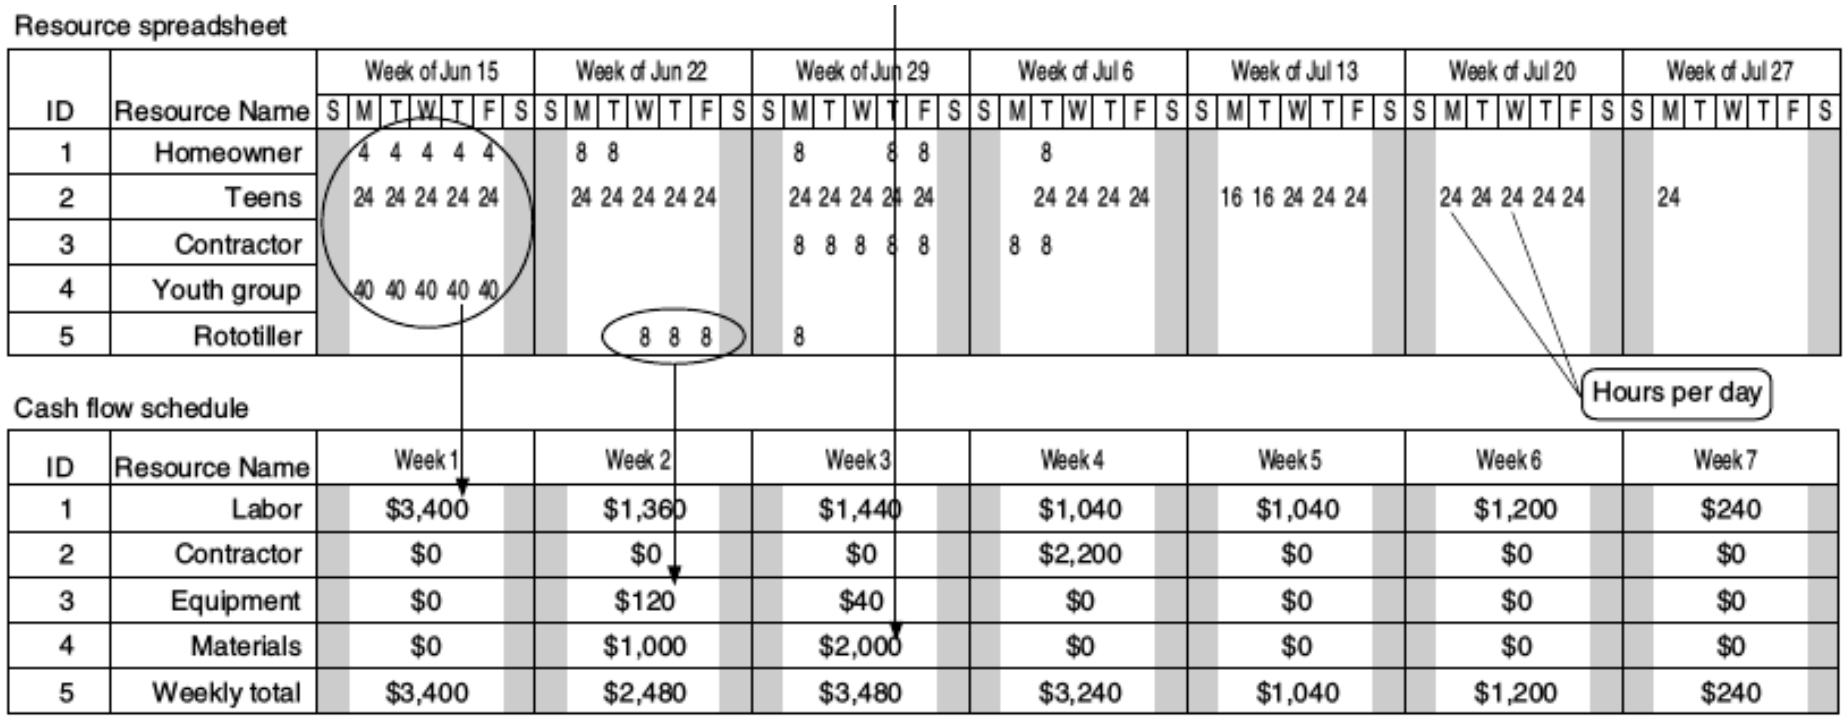
\includegraphics[width=0.95\textwidth]{cashFlow.png}
\end{center}

При планировании денежных потоков вы определяете, когда и сколько денег поступит или будет уплачено по счетам, чтобы обеспечить нормальную деятельность предприятия. При этом необходимо учесть возможный временной сдвиг между реальным заключением договора и фактическим получением денег. В начале проекта вы скорее всего получите лишь небольшой аванс, а остальные деньги будете получать частями по достижении заранее оговоренных ключевых точек, либо, в худшем случае, в самом конце, когда проект будет завершён. Ну и надо понимать, что банковский перевод от заказчика к вам и от вас к сотрудникам тоже занимает время, а люди привыкли получать зарплату примерно в одно и то же время, и могут расстроиться, если будут осуществляться задержки.

\section{Отслеживание прогресса}

Теперь поговорим про управление проектами и действия, которые менеджер проекта может (и должен) совершать в ходе проекта. PMBOK определяет целый набор разных видов деятельности (см. рисунок ниже), мы же продолжим говорить про треугольник равновесия проекта и способы балансирования этого равновесия.

\begin{center}
    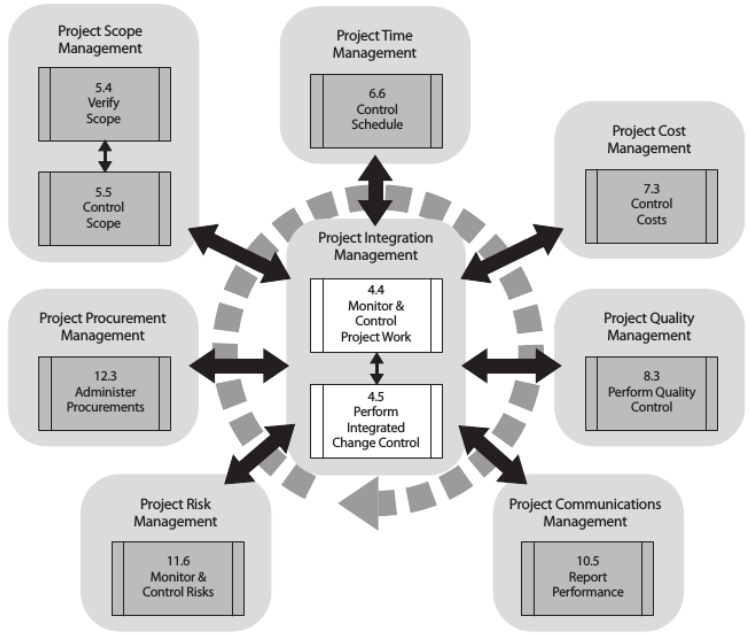
\includegraphics[width=0.6\textwidth]{pmbokProjectManagement.png}
\end{center}

\subsection{Балансирование равновесия проекта}

\subsubsection{Треугольник равновесия}

В каждом проекте есть три основных момента:

\begin{itemize}
    \item стоимость;
    \item ресурсы (люди, компьютеры, время...);
    \item функциональность.
\end{itemize}

\begin{center}
    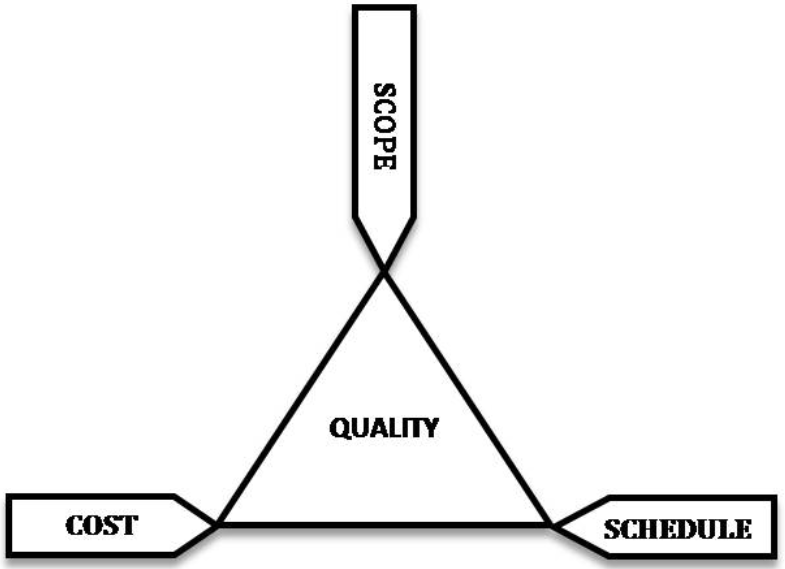
\includegraphics[width=0.4\textwidth]{balanceTriangle.png}
\end{center}

Если вы измените одну из этих переменных, то это неизбежно отразится и на оставшихся переменных тоже. Действительно, если вы увеличите функциональность вашего проекта (добавите новые фичи), то вы не сможете это сделать с той же стоимостью за то же самое время. Это очевидно, поскольку у вас работы больше стало. Если у вас становится меньше денег или людей, то это, разумеется, скажется на качестве продукта, вы не реализуете то же самое количество функциональности за то же самое время. Точно так же, чтобы обеспечить такое же качество продукта за более короткий период времени, придется увеличить стоимость. Задача менеджера проекта, состоит в том, чтобы сбалансировать эти переменные, чтобы создать оптимальное равновесие между ценой и качеством.

Есть еще одна интересная картинка~--- то же самое, но для заказчика:

\begin{center}
    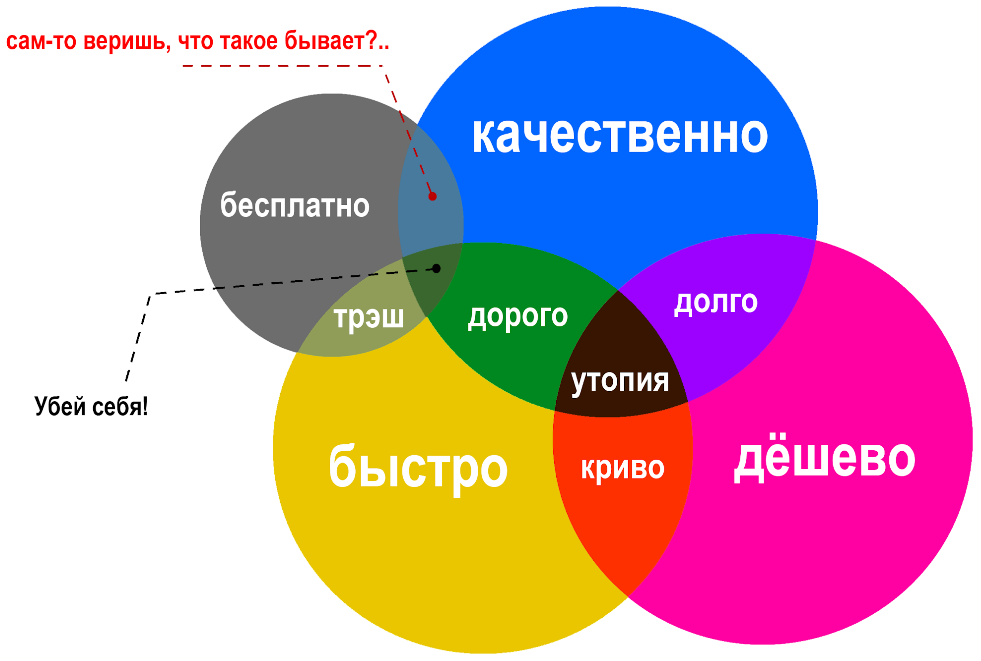
\includegraphics[width=0.6\textwidth]{balanceTriangleExplained.png}
\end{center}

Не бывает быстро, качественно и дешево. Если вы делаете быстро и дешево~--- получается криво; дешево и качественно~--- долго; быстро и качественно~--- дорого и т.д.

Равновесие в проекте нужно сохранять постоянно (до завершения работы над проектом). Эта работа делается на разных уровнях: проекта, бизнес-целей, компании.

\paragraph{Балансирование на уровне проекта.} Изменения, которые никак не повлияют на сроки, бюджет, количество людей и т.д., менеджер может принимать сам, они не требуют авторизаций или разрешений. Пока это остается в рамках ограничений, с проектом можно делать всё, что угодно.

\paragraph{Балансирование на уровне бизнес-целей.} Изменения на уровне проекта возможны не всегда, иногда их просто недостаточно, и требуется сдвигать одну или несколько вершин треугольника равновесия. В таком случае нужно принимать решения на уровне бизнес-целей, а это требует согласования с заказчиком и/или руководством компании.

\paragraph{Балансирование на уровне компании.} Изменения на уровне компании~--- глобальные изменения. Подобные изменения принимаются уже руководством компании, которое должно балансировать сразу все проекты компании. Например, у одного проекта может быть резко урезан бюджет с целью выделения дополнительных средств другому, более критичному проекту. Данный уровень в лекции мы затрагивать не будем.

\subsubsection{Балансирование на уровне проекта}

\paragraph{Повторная переоценка задач.} Первое, что стоит попробовать сделать при балансировке на уровне проекта~--- повторно оценить задачи. То есть, уже в процессе работы ещё раз пересмотреть график проекта и задачи в нем. Возможно сейчас у вас больше информации, чем на этапе изначальной оценки, и оценки получатся точнее. Вполне возможно, какие-то задачи были переоценены, а некоторые вообще уже потеряли актуальность.

Однако при переоценке задач следует действовать очень осторожно: нельзя выдавать желаемое за действительное. Например, если хочется сократить бюджет, то возникает большой соблазн обмануться и избавиться от задач, которые на самом деле важны.

Плюсы: потенциальное сокращение сроков, бюджета, объема работ. Но если новой информации или требований у вас не появилось, то этот метод вряд сильно сработает. Тем не менее, к нему стоит время от времени возвращаться.

\paragraph{Перераспределение задач критического пути.} При балансировании проекта всегда стоит уделять особое внимание задачам на критическом пути в сетевом графике.

Можно попробовать увеличить число людей, занятых работой над критическими задачами, задавшись целью сделать их быстрее. Обычно привлекают людей, работающих над другими задачами. Однако, такой подход может скрывать массу подводных камней. Во-первых, добавление людей к задаче не всегда повышает продуктивность работы, например, если задачи были распланированы с оптимальным количеством людей. Кроме того, следует иметь в виду, насколько хорошо задачи параллелятся. Если хорошо, то добавление новых людей к решению этой задачи, скорее всего, принесет пользу. Но чаще всего задачи нельзя распараллелить. Например: задача разработки архитектуры, запланированная на одного архитектора, не будет сделана существенно быстрее архитектором и четырьмя программистами. Добавление людей к таким задачам в худшем случае только замедлит работу, а в лучшем~--- принесёт незначительное улучшение.

Следует также иметь в виду, что при привлечении новых людей к решению задачи продуктивность каждого из работников может упасть. Соответственно, расходы проекта растут. Ну и при переводе человека из одного проекта в другой может потребоваться время на его обучение и адаптацию.

Таким образом, при перераспределении людей по задачам нужно учитывать следующие моменты.

\begin{itemize}
    \item Квалификация работников: не стоит заставлять дизайнера писать тесты или проектировать архитектуру.
    \item Действительно ли это поможет сократить время работы? Не будет ли человек лишним? 
    \item Как поменялись резервы в задачах? Не изменился ли критический путь?
\end{itemize}

\paragraph{Добавление людей в проект.} При добавлении людей в проект задачи практически никогда не начинают резко делаться быстрее, чем до этого, т.к. при добавлении человека в уже запущенный проект его нужно хотя бы как-то обучить и адаптировать, контролировать его работу. Это приводит к трате времени других людей в проекте, соответственно, сбивается график проекта: человек, который мог бы в это время делать задачи проекта, тратит своё время на нового сотрудника (а сам новый сотрудник ещё не работает). В графике продуктивности команды при добавлении новых людей почти всегда происходит сначала небольшой спад.

Исходя из этого, в краткосрочной перспективе добавление новых людей в проект невыгодно (только если добавляется не какой-нибудь супер-специалист, который хорошо знает команду, предметную область и проект). Почти всегда добавление новых людей~--- это инвестиция в будущее проекта.

Резервы для добавления обычно ищутся внутри компании, но обычно из резерва можно найти не самых опытных людей. Поэтому не стоит надеяться на то, что в критической ситуации можно резко добавить ещё крутых специалистов, и всё пойдёт быстрее.

Привлечение новых людей хорошо работает в проектах с открытым исходным кодом, поскольку в подобных проектах, как правило, обычно строго древовидная иерархия и с новым человеком работает локальная часть этой иерархии. Однако, например, в agile проектах это может работать хуже, поскольку новый человек будет обращаться за помощью ко всем (т.к. может) и тем самым затормозит прогресс проекта. О том, как подобный подход может разрушить планы даже очень крупных компаний, можно почитать, например, тут: \url{https://www.eurogamer.net/stormlands-and-the-million-man-raid-obsidians-cancelled-xbox-one-exclusive} (дата обращения: 27.03.2023).

\paragraph{Привлечение экспертов в проект.} Эксперты бывают внутренние (изнутри компании) и внешние.

Внутренний эксперт~--- специалист внутри компании, временно снятый со своего основного проекта. Такой эксперт привлекается, как правило, чтобы помочь с какой-то локальной проблемой, а потом вернуться к своей основной работе. Плюсы: человек лоялен к проекту/компании, обладает требуемыми компетенциями и готов их вам предоставить в лучшем виде. Например, эксперт настраивает базу данных, делает это быстро и грамотно, время внутри команды не тратится. Но, во-первых, эксперт~--- человек, он тоже может совершить ошибку при настройке, может не уложиться в сроки и т.д. Во-вторых, никаких компетенций в области конкретной задачи, для решения которой привлекли эксперта, командой проекта не приобретается, т.к. всё сделал сторонний человек.

Что же делать, если снова случится такая проблема? Если бы было потрачено время на обучение своего сотрудника, то при необходимости этот сотрудник мог бы снова решить проблему. Таким образом, в долгосрочной перспективе лучше обучать своих специалистов.

С целью избежания подобных ситуаций (а также с целью повышения компетенций команды) при привлечении эксперта со стороны, его нужно заставить передавать знания. Вряд ли это будет встречено с охотой, но неким образом эксперт всё же должен быть вовлечён в процесс планирования. Можно заставить эксперта участвовать в статус-митингах, попросить провести семинар и т.д. В таком случае привлечение эксперта работает хорошо, и при возникновении проблемы, схожей с той, для решения которой был привлечён эксперт, команда проекта уже будет иметь хотя бы некоторые знания, связанные с решением возникшей задачи.

Внешний эксперт~--- то же самое, но с компетенциями всё обстоит ещё хуже, поскольку это полностью сторонний человек, которого можно попросту не найти, если вдруг проблема возникла снова (или же при решении были допущены ошибки).

Предпочтительный вариант~--- растить собственных экспертов. Это осуществляется либо с привлечением внутренних экспертов компании, либо же приглашением людей со стороны, которые будут обучать членов команды. Следует специализировать людей внутри команды в конкретных областях. Со временем они вполне сами могут стать экспертами (если не уйдут от вас в другой проект).

\paragraph{Аутсорсинг частей проекта.} Аутсорсинг~--- передача части проекта на разработку сторонней компании. При подобном подходе возникают две проблемы: помимо неприобретённой экспертизы, вы получаете зависимость от сторонней компании. Можно даже не догадываться, что происходит в той компании, которой отдана часть проекта, и у менеджера проекта существенно меньше возможностей контролировать процесс разработки. Аутсорсинг~--- довольно экстремальная вещь: или всё идёт хорошо, или всё идет плохо, а команда об этом и не подозревает. Нужно стараться контролировать процесс выполнения работы над частью проекта, отданной \enquote{на растерзание} другой компании. Из очевидных плюсов, аутсорсинг позволяет избежать проблем с квалификациями своих разработчиков. Например, когда нужно сделать приложения под все платформы, а программистов под iOS в команде нет, и заводить их не хочется. В таком случае аутсорсинг~--- очень выгодное решение.

\paragraph{Сверхурочная работа.} Ещё один часто приходящий на ум вариант повышения продуктивности~--- заставить членов команды работать больше. Казалось бы, всё выглядит очень оптимистично: пусть есть $X$ часов в неделю суммарно при работе программистов по $40$ часов. Если заставить их работать по $60$ часов в неделю, получим $1.5 * X$. Кроме того, не нужно добавлять новых людей, обучать их и т.д., просто члены команды будут работать дольше. Да и дополнительное время они будут работать в нерабочее время, когда офис не так сильно заполнен людьми, так что будут меньше отвлекаться и т.п.

Однако, на самом деле всё вовсе не так хорошо. Конечно, это нормально, если перед дедлайном приходится, например, поработать в выходные, чтобы сделать релиз в понедельник, но если переработки происходят регулярно, то программисты начинают \enquote{выгорать}. Люди начинают уставать, продуктивность падает. Но мы про это уже говорили в одной из прошлых лекций.

При решении интеллектуальных задач производительность очень сильно страдает от усталости. Заставить человека, занимающегося интеллектуальным трудом, работать больше, чем обычно~--- почти всегда путь к плохим последствиям. Как писал ДеМарко, на каждый час переработки приходится примерно час недоработки. И это он ещё оптимист. Не бывает так, чтобы люди волшебным образом стали работать в 1.5-2 раза больше. Фанатизм в работе сказывается на здоровье, усталости. Заканчивается это часто возросшей апатией человека и нежеланием делать вообще что-либо. Таким образом очень легко теряются программисты. В долгосрочной перспективе переработки крайне невыгодны.

Грамотный менеджер должен не заставлять команду программистов работать \enquote{на часик подольше}, а как раз наоборот, следить за тем, чтобы не было систематических переработок. Сознательные переработки~--- признак непрофессионализма. Если человек каждый день засиживается на работе, то, скорее всего, у него проблемы с тайм-менеджментом. Скорее всего, в течение дня он тратит свое время на что-то никак не связанное с работой. Здесь, опять же, бывают исключения, но таких людей (\enquote{фанатиков}) очень мало, и с ними, как правило, всё понятно. И они тоже выгорают.

\paragraph{Снижение качества проекта.} \emph{Качество проекта никогда не следует понижать.} Конечно, соблазн велик, но последствия всегда весьма плачевны. Например, можно сэкономить на тестах, но взамен поймать кучу рандомных багов. Даже в краткосрочной перспективе не стоит понижать качество продукта, т.к., скорее всего, будет сделан очень некачественный продукт, который потом придется переделывать, на что уйдет больше времени, особенно если это придётся делать через несколько месяцев после завершения работы. Возможно даже, что придется переписывать весь проект заново. Гораздо дешевле не допускать ошибок, чем их исправлять. Жертвовать можно чем угодно, но не качеством. Даже если вы сдадите проект, потерянную репутацию потом будет крайне сложно восстановить.

\subsubsection{Балансирование проекта на уровне бизнес-целей}

\paragraph{Пересмотр границ проекта.} Когда приходит понимание, что в заданные сроки и бюджет требуемую функциональность реализовать не получается, стоит посмотреть, а нельзя ли как-то подвинуть границы проекта, нельзя ли от какой-то функциональности более-менее безболезненно избавиться (хотя бы на данном этапе). Подобные решения требуют обоснованных переговоров с заказчиком и часто основываются на анализе требований и сценариев использования продукта. Поэтому их можно осуществлять только на уровне бизнес-целей компании. Ну и не всегда можно безболезненно выбросить какую-то функциональность: всё же продукты должны обладать какими-то особенностями, чтобы иметь на рынке конкурентное преимущество. А такие особенности чаще всего и являются тем, что сложно в реализации (иначе у конкурентов оно уже было бы тоже реализовано).

\paragraph{Подстраивание проекта под дедлайны.} Часто бывает так, что у продуктов есть фиксированный дедлайн, в который команда не укладывается, однако дедлайн имеет первостепенную важность. В таком случае следует разбить период времени до дедлайна на несколько этапов, по завершении каждого из которых будет согласовываться дальнейшее направление развития проекта. В каждой ключевой точке фиксируется функциональность на ближайший этап, при достижении следующей планируется следующий этап и т.д. В итоге набор функциональности можно определять динамически.

Подобный подход работает далеко не всегда. Например, заказчик может захотеть добавить что-то, что просто не вписывается в текущую архитектуру. Также заказчик может хотеть работать по более традиционной схеме и отказаться брать на себя ответственность за разбиение проекта на этапы и определение функциональности на них.

\paragraph{Работа на опережение.} Для работ, которые нельзя сделать параллельно, можно применить следующий подход. Допустим, у нас есть задача A, а также задача B, которая должна быть сделана по завершении работы над задачей A. В таком случае можно начать делать B ещё до завершения A. Например, можно начать реализовывать отдельные компоненты проекта до того, как архитектура будет закончена целиком.

При таком подходе надо действовать аккуратно, т.к. есть большая вероятность того, что придется переделывать решение. Это связано с тем, что принимаются предположения касательно реализации в духе \enquote{скорее всего, это будет так}, однако гарантии этого нет и в результате всё может быть совсем иначе.

Если всё сложится удачно, данный подход может позволить получить хорошую выгоду, но возможен и негативный исход, который приведет к уходу в минус. Тем не менее, при грамотном анализе рисков подобная \enquote{хитрость} может помочь. С помощью такой техники можно сэкономить до 30-40\% времени.

\paragraph{Incremental delivery.} Поэтапная разработка: поставлять заказчику изменения в продукте небольшими партиями. Такой подход работает далеко не со всеми проектами (и уж тем более не со всеми заказчиками). Например, это точно не сработает с большими, монолитными системами. Но, как правило, такое бывает довольно редко, а вот заказчики, которые не хотят так работать, встречаются весьма часто. Мы это уже подробно обсуждали в лекциях про гибкие модели разработки.

\paragraph{Прототипирование.} Прототипирование~--- мощный инструмент, суть которого заключается в том, что до начала работы над проектом создается черновой вариант проекта целиком (или каких-то его частей), но без особого внимания к качеству и деталям. Такой прототип создается просто для теста и получения опыта/знаний о предметной области, поэтому, когда работа над ним завершена, нужно избавиться от него и сделать заново, но уже хорошо.

Этот подход вынуждает потратить больше денег на разработку (приходится делать многое дважды), но, с другой стороны, позволяет снять риски и потратить меньше денег на исправление ошибок. Следует отметить, что очень важно избавиться от первоначального прототипа по завершению его разработки, а не использовать его в качестве основания для \enquote{настоящего} проекта, поскольку прототип, как уже было сказано выше, делается на скорую руку и, скорее всего, будет целиком и полностью основан на \enquote{костылях}.

\paragraph{Снижение прибыльности проекта.} Пожертвовать прибыльностью проекта~--- последний шаг, к которому стоит прибегнуть, если ничего больше не работает. Это подразумевает уход проекта \enquote{в минус}, заём денег у других проектов, и т.д. Другой вариант~--- жертвовать репутацией и выпускать продукт ненадлежащего качества, позже дедлайна, и т.д. Далеко не все компании согласны на такое, поэтому чаще прибегают к потери прибыли проекта, но сохранению репутации.

\subsection{Отслеживание прогресса проекта}

Для того, чтобы уметь адекватно управлять ходом проекта, менеджер должен постоянно отслеживать кучу самых разных характеристик проекта.

\subsubsection{Задачи}

Например, следует почаще заглядывать в таск-трекер, и делать соответствующие выводы: сколько задач открыто, сколько закрыто, переоткрыто за какой-либо период; какое среднее количество дней до завершения задачи; среднее время переработок/недоработок по задачам; и т.д.

Это очень важная информация, которую стоит накапливать и отслеживать тренд изменений. Лучше всего нарисовать графики для каждой из наиболее важных метрик, это позволит понять события, происходящие в проекте, более детально. Например, если количество переоткрытий задач растет, нужно уделить больше внимания качеству и ревью, и т.д. 

Следует стараться делать задачи небольшими, иначе отслеживать их прогресс будет очень сложно. У каждой задачи должен быть очевидный критерий завершенности, чтобы однозначно определять, когда задачу можно закрыть.

Помимо таск-трекера источником подобной информации являются регулярные статус-митинги. Они также помогают отслеживать прогресс, но более направленно и субъективно. Например, человек не будет писать о сложностях, которые у него возникли при работе, в комментариях к своей задаче, но при разговоре он об этом, скорее всего, скажет.

\subsubsection{Люди}

Из таск-трекера также можно извлечь много информации персонально по поводу каждого конкретного разработчика. Сколько задач конкретный человек сделал, сколько переоткрыл, сколько сейчас на нём висит, переработка/недоработка, и т.д. Например, если у программиста недоработки и большое количество переоткрытых задач, то, скорее всего, он работает неэффективно и нужно привлечь его внимание к этому вопросу.

Также хорошей практикой являются еженедельные отчеты. Обычно они оформляются в виде таблички, в которой указаны задачи, которыми человек занимался, и количество часов на каждую. С таким видом статистики следует быть осторожным, т.к. на практике менеджер часто хочет увидеть в этой табличке строго 40 рабочих часов за неделю. Не стоит так делать, поскольку если заставить людей писать \enquote{40}, то они и будут писать \enquote{40}, а такая статистика вряд ли будет соответствовать действительности, т.к. люди будут подгонять время под это количество часов. Как показывает практика, в реальной жизни получается не 8 часов в день, а немного меньше. Поэтому, если проект идет по графику и результат получается хорошим, то 40 часов в неделю может и не быть (и это не страшно). Фраза \enquote{должно быть 40} всегда всё портит. Если же этого избегать, то программисты не будут пытаться натянуть свой график на эти мифические 40 часов. Соответственно, оценки будут честные.

Следует также сказать, что написание отчетов дисциплинирует программистов (несмотря на то, что они будут этому активно сопротивляться), а для менеджера такие отчеты очень важны для сбора и анализа данных. Если есть возможность генерации подобных отчетов из таск-трекера вместо ручного заполнения~--- это большой плюс.

\subsubsection{Дефекты}

Аналогично людям и задачам, только по известным ошибкам и прочим дефектам: общее количество дефектов, относящихся к сотруднику; количество незакрытых дефектов, относящихся к сотруднику; среднее время исправления дефекта; процент переоткрытых дефектов; распределение дефектов по модулям/компонентам, приоритетам, статусам; количество дефектов для каждой задачи  и т.п.

\subsubsection{Коммиты}

При оценке производительности программиста по коммитам важно учитывать многие факторы. Во-первых, важно не количество коммитов, а их содержательная часть. Просто считать коммиты или количество измененных строчек~--- не лучший подход, поскольку изменения бывают разные (например, можно просто заменить все пробелы в проекте на символы табуляции. Количество строчек будет огромным, а их практическая ценность нулевой). У всех разный стиль разработки, но всё же обычно есть общепринятая культура в команде, так что интересно смотреть на время коммитов, их регулярность.

\subsubsection{Графики}

При анализе каких-то численных показателей следует смотреть на общую динамику изменений. Не стоит смотреть на цифры в отдельности, т.к. это не слишком наглядно.

Например, рассмотрим два графика: по планируемой/выполняемой работе и по затратам:

\begin{center}
    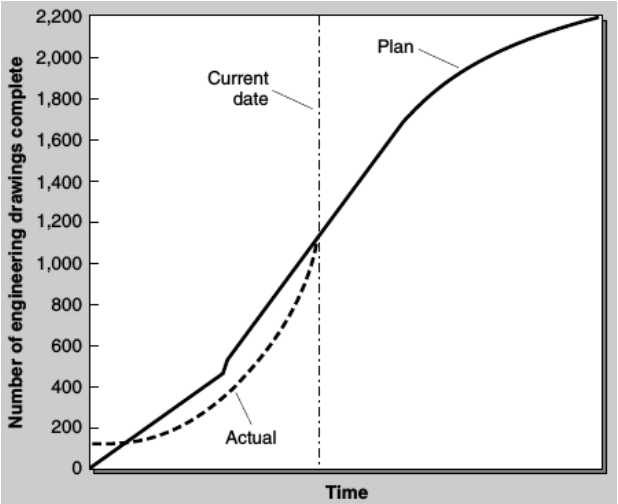
\includegraphics[width=0.5\textwidth]{plannedWorkGraph.png}
\end{center}

\begin{center}
    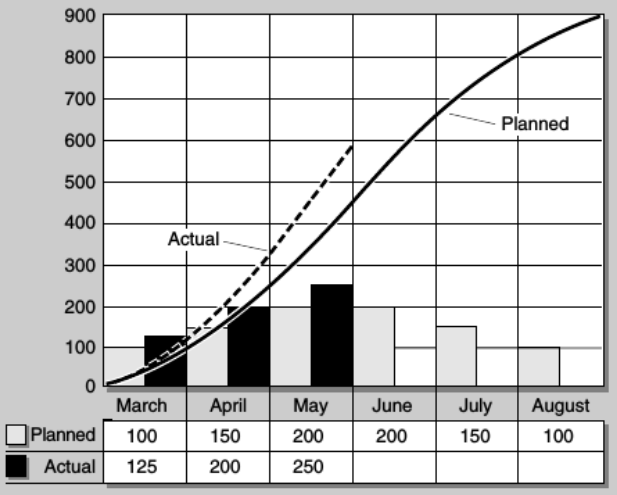
\includegraphics[width=0.5\textwidth]{costGraph.png}
\end{center}

Оба графика показывают изменение показателей во времени, но у них есть свои недостатки. Первый график плох тем, что в нем не учитывается сложность задач. Он показывает лишь то, что команда отстает, а в какой-то момент догоняет исходный план. Но это не показывает, какие задачи были сделаны~--- возможно, самые простые, а может быть и самые сложные.

Второй график~--- график расходов~--- показывает, что команда тратит больше, чем нужно, но, возможно, было выполнено гораздо больше запланированной работы.

Для полноты картины нужно смотреть на происходящее в проекте со всех сторон, иначе особого смысла нет. Без контекста подобную информацию можно с лёгкостью интерпретировать неверно.

Ещё некоторые показатели:

\begin{itemize}
    \item Budgeted Cost of Work Scheduled (BCWS)~--- планируемая стоимость работ на данный момент времени;
    \item Budgeted Cost of Work Performed (BCWP)~--- плановая стоимость выполненных на данный момент работ;
    \item Actual cost of work performed (ACWP)~--- реально израсходованный бюджет;
    \item Cost variance (CV) $= BCWP - ACWP$~--- разница между планом и реальными расходами;
    \item Cost variance percent (CV\%) $= CV / BCWP$~--- то же самое, но в процентах;
    \item Cost performance index (CPI) $= BCWP / ACWP$~--- индекс производительности (если меньше единицы~--- тратится больше, чем запланировано, больше~--- тратится меньше);
    \item Estimate budget at completion (EAC) $= BAC / CPI$~--- планируемая стоимость всего проекта;
    \item Budget at completion (BAC)~--- итоговая стоимость всего проекта;
\end{itemize}

Какие-то из этих или другие интересующие показатели тоже имеет смысл отслеживать на графиках:

\begin{center}
    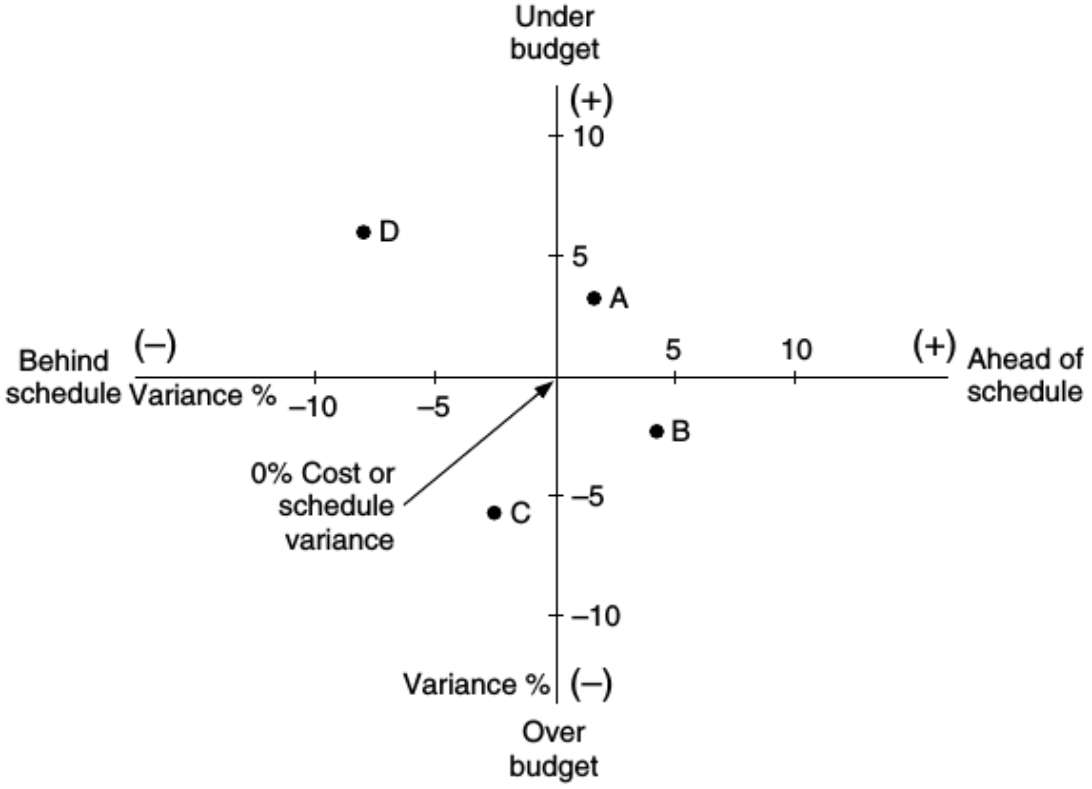
\includegraphics[width=0.6\textwidth]{varianceGraph.png}
\end{center}

Более интересный график пытается учитывать одновременно и время, и деньги:

\begin{center}
    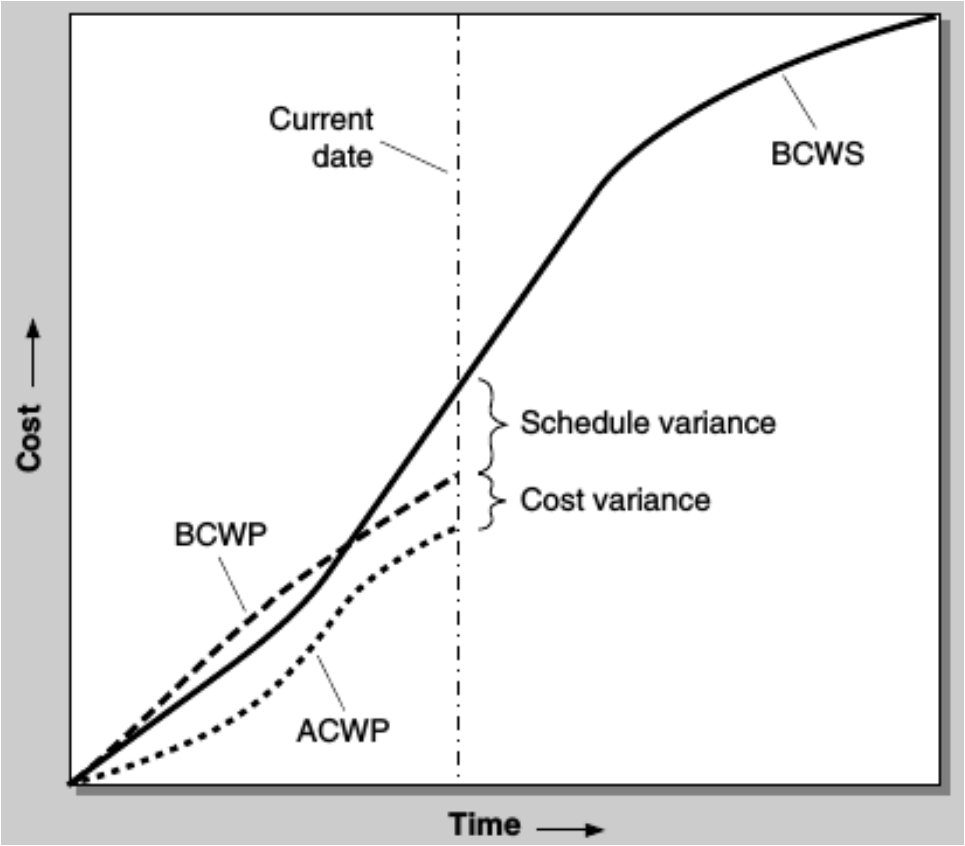
\includegraphics[width=0.5\textwidth]{metricsGraph.png}
\end{center}

На горизонтальной оси тут отклонение по времени, на вертикальной~--- по затратам. Например, первый квадрант~--- проект идёт с опережением времени и бюджета, третий квадрант~--- отставание по времени и перерасход бюджета.

На этом же графике полезно отмечать критические пороги значений параметров, при которых имеет смысл обозначить проблему перед начальством:

\begin{center}
    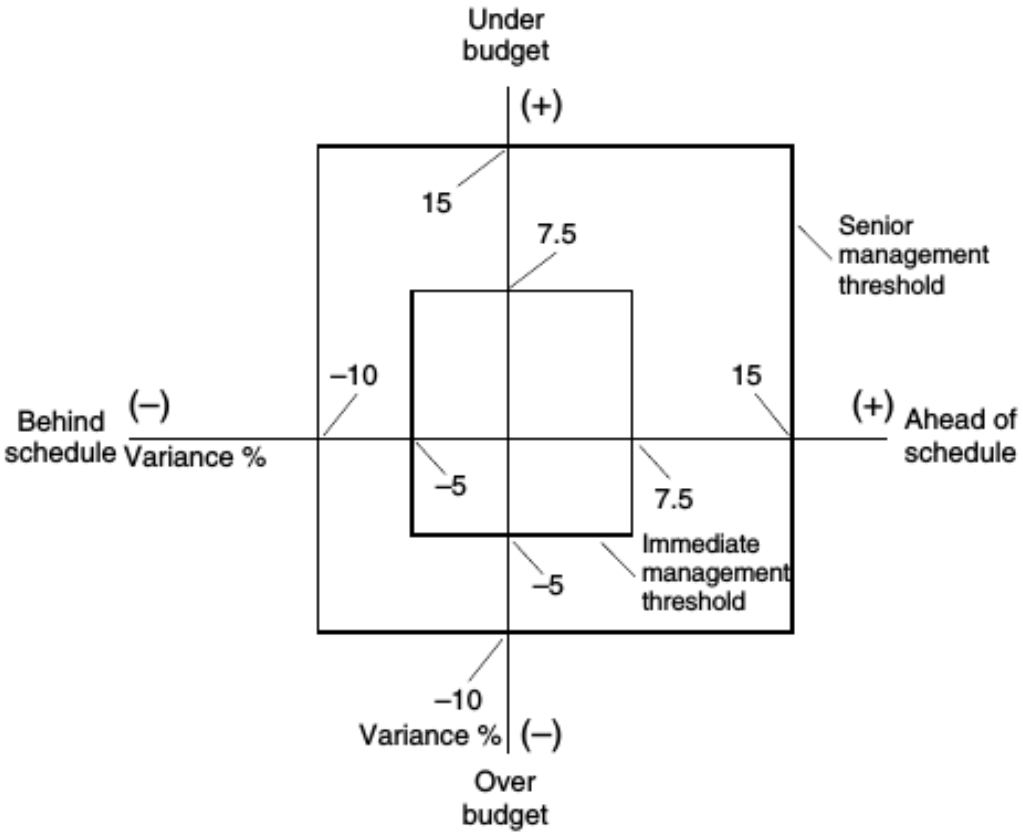
\includegraphics[width=0.6\textwidth]{escalationThresholds.png}
\end{center}

Границ может быть несколько в зависимости от критичности значений, и они позволяют более осознанно принимать проектные решения самостоятельно или определять момент, когда уже пора таки обратиться за помощью. 

\end{document}
